\scanpage{15}
\mspage{13}

g manifestement se prolonge en $\overline{g}$ : $\overline{T}\rightharpoondown XxY$ . Cela nous ramène à prouv
que \inserted{le composé} \handwritten{(}$\handwritten{\unsure{t|\dagger}\,\unsure{i}}\overline{T}'\xrightarrow{\handwritten{\alpha_i}}\handwritten{\unsure{t|\dagger|F}}Z'_i\overset{\handwritten{\alpha_{i\unsure{*}}}}{\rightharpoondown}\handwritten{\unsure{t|\dagger}}\overline{T}'$ ne dépend pas de i=0,1. Ecrivons X au lieu de $\overline{T}'$, \unsure{'}

considérons le diagramme cartésien d'inclusions
\diagram{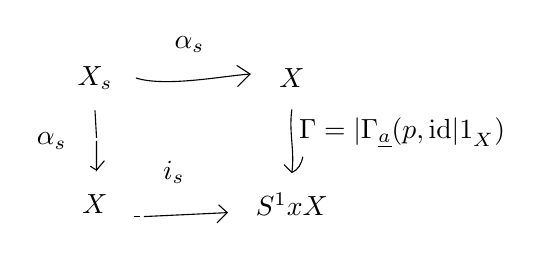
\begin{tikzpicture}[x=1cm,y=1cm,baseline] \node at (0,1.6) {$X_s$}; \node at (2.5,1.6) {$X$}; \node at (0,0) {$X$}; \node at (2.5,0) {$S^1xX$}; \node at (1.2,2.02) {$\alpha_s$}; \node at (-.55,.8) {$\alpha_s$}; \node at (1,.4) {$i_s$}; \node at (3.9,.9) {$\unsure{\Gamma=|\Gamma_{\underline{a}}}\unsure{(}p,\unsure{\mathrm{id}|1}_X)$}; \draw (.52,1.6) .. controls (.9,1.48) and (1.65,1.63) .. (1.97,1.65); \draw (1.8,1.76) -- (1.97,1.65) -- (1.81,1.49); \draw (0,1.19) -- (.02,.84); \draw (.02,.8) -- (.02,.43) -- (.12,.55); \draw (.02,.43) -- (-.06,.48); \draw (2.5,1.2) .. controls (2.46,.9) and (2.54,.68) .. (2.5,.4); \draw (2.4,.5) -- (2.5,.4) .. controls (2.57,.42) and (2.63,.52) .. (2.64,.6); \draw (.49,-.16) -- (.57,-.16); \draw (.62,-.16) -- (1.68,-.11); \draw (1.57,-.01) -- (1.68,-.11) -- (1.55,-.24); \end{tikzpicture}},

on a alors $\handwritten{\alpha}^{\handwritten{*}}_s\,\handwritten{\unsure{\alpha}}_{s*}=\handwritten{\Gamma}^{\handwritten{*}}i_{s\handwritten{\unsure{*}}}$ , qui ne dépend pas de s puisque $i_s$ n'en
dépend pas à homotopie près. - Le reste est sans doute l'AQT.

Sur la strcture des B.(X). Ce sont tous des algèbres graduées
sur B.(pt)=\handwritten{$\Lambda$} , qui est une algèbre graduée à degrés positifs, réduit
\margin{\figure{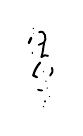
\begin{tikzpicture}[x=.5em,y=.5em,line cap=round,line join=round]
\fill (.38,6.15) circle (.055);
\fill (.40,5.78) circle (.03);
\draw[line width=.7pt] (.80,5.88) .. controls (1.23,6.08) and (1.37,5.37) .. (1.15,5.11) .. controls (1.10,4.75) and (1.05,4.31) .. (.96,4.08) .. controls (1.12,4.25) and (1.29,4.23) .. (1.44,4.17);
\draw[line width=.65pt] (1.18,5.14) -- (.76,4.96);
\draw[line width=.9pt] (.22,5.46) -- (.06,5.10);
\fill (.31,4.38) ellipse (.055 and .09);
\draw[line width=.8pt] (.87,3.68) .. controls (.61,3.40) and (.45,3.04) .. (.37,2.75) .. controls (.45,2.65) and (.53,2.64) .. (.64,2.63);
\fill (1.12,3.02) circle (.045);
\draw[line width=.7pt] (1.72,3.30) .. controls (1.84,3.04) and (1.71,2.88) .. (1.59,2.74);
\fill (1.29,2.34) circle (.05);
\fill (1.38,1.84) circle (.05);
\draw[line width=.65pt] (.72,1.72) .. controls (.83,1.67) and (.94,1.67) .. (1.02,1.67);
\fill (1.55,1.23) circle (.04);
\fill (1.22,.88) ellipse (.07 and .10);
\fill (1.11,.50) circle (.055);
\end{tikzpicture}}}
à $\underline{F}_2$ en degré\deleted{\unsure{z|s}} 0. C'est d'ailleurs une algèbre de polynômes \inserted{\begin{tabular}[b]{@{}l@{}}\handwritten{à une infinité de générateurs $X_i$ ($i$ entier \unsure{$\geq|>$} \illegible{2}}\\[-.6ex]\begin{tikzpicture}[x=.6cm,y=.6cm,baseline] \draw (.12,.45) .. controls (-.2,.13) and (-.13,-.06) .. (.12,-.15) .. controls (.32,-.21) and (.5,-.2) .. (.76,-.29); \end{tikzpicture}\end{tabular}} connue\,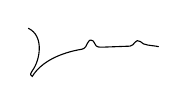
\begin{tikzpicture}[x=.65cm,y=.65cm,baseline] \draw (0,.45) .. controls (.32,.3) and (.23,-.18) .. (.08,-.38) .. controls (.05,-.44) and (.02,-.45) .. (.08,-.49) .. controls (.25,-.21) and (.62,-.03) .. (1.05,.04) .. controls (1.19,.07) and (1.13,.28) .. (1.27,.2) .. controls (1.34,.1) and (1.3,.08) .. (1.45,.08) -- (1.99,.1) .. controls (2.08,.11) and (2.09,.26) .. (2.19,.19) .. controls (2.25,.11) and (2.4,.12) .. (2.55,.09); \end{tikzpicture}
On a un homomorphisme évident \inserted{d'anne\unsure{\deleted{d}a|\deleted{a}d}\unsure{\deleted{t}u|\deleted{u}t}xp\unsure{\deleted{d}g|\deleted{g}d|g}\unsure{\deleted{i}r|\deleted{r}i}adués} B.(X) $\to H^{\handwritten{\unsure{B}}}(X)$, nul en degrés \handwritten{$>$}0, qui
\margin{\handwritten{\uline{NB} $H^*(X)$ $(=H^*(X,\mathbb{F}_2)$}}
à tout Z sur X associe l'image de 1 \handwritten{$\in$} $H^o(Z)$ par l'homomorphisme de Gys
\margin{\handwritten{en fait $H(X)\simeq B.(X)/\Lambda^+B.(X)$}}
associé à Z$\to$ X. Cet homomorphisme par Thom est surjectif (toute cla
se de cohomologie provient d'une image de variété compacte....); \deleted{\unsure{n}ote}

On ppouve même qu'il existe un relèvement fonctoriel en X
\margin{\handwritten{?}}
$H^\bullet$(X) $\to$ B.(X), \inserted{\begin{tabular}[b]{@{}l@{}}\handwritten{il est douteux qu'il soit}\\[-.6ex]\begin{tikzpicture}[x=1.35cm,y=.6cm,line width=.4pt]\draw (.11,.67)..controls(-.15,.24)and(-.13,-.37)..(.05,-.47);\draw (.21,-.25)..controls(.30,-.18)and(.42,-.14)..(.58,-.14);\draw (.62,-.14)--(.72,-.14);\draw (.78,-.14)--(.82,-.14);\draw (.89,-.14)--(.94,-.14);\draw (1.00,-.14)--(1.02,-.14);\draw (1.12,-.14)--(1.13,-.14);\draw (1.17,-.14)--(1.18,-.14);\draw (2.61,-.16)--(2.64,-.16);\draw (2.71,-.16)--(2.73,-.16);\draw (2.80,-.16)--(2.82,-.16);\draw (3.49,-.14)--(3.51,-.14);\draw (3.58,-.14)--(3.65,-.14);\draw (3.74,-.14)--(3.84,-.13);\draw (3.92,-.13)--(3.96,-.13);\draw (4.04,-.12)--(4.06,-.12);\draw (4.3,.64)..controls(4.35,.24)and(4.36,.12)..(4.08,.03);\end{tikzpicture}\end{tabular}} compatible avec multiplication\handwritten{)} \deleted{t\unsure{e}l}tel que l'on ait:

\deleted{a)} L'homomorphisme correspondant $H^\bullet(X)\otimes_{\underline{F}_2}\handwritten{\Lambda}\simeq$ B.(X) est un iso
\margin{\handwritten{?}}
morphisme (ce sera vrai pour tout relèvement individuellement ...), e

\deleted{b)}\handwritten{[}\deleted{Le}\inserted{\begin{tabular}[b]{@{}l@{}}\handwritten{Quillen ignore si}\\[-.6ex]\begin{tikzpicture}[x=1cm,y=.6cm,line width=.4pt]\draw (.08,-.25)..controls(.01,-.12)and(-.03,.04)..(-.03,.14);\draw (-.03,.25)--(-.03,.33);\draw (-.02,.42)--(.01,.53);\draw (.04,.59)--(.10,.66);\draw (.15,.70)--(.34,.76);\draw (.40,.78)--(.44,.79);\draw (2.35,.75)--(2.43,.75);\draw (2.50,.75)--(2.58,.74);\draw (2.64,.74)--(2.82,.73);\draw (2.89,.73)--(2.96,.73);\draw (3.05,.72)--(3.26,.71);\draw (3.40,.70)--(3.68,.69);\draw (3.77,.69)--(3.98,.68);\draw (4.08,.68)..controls(4.56,.71)and(4.65,.85)..(4.65,1.02);\end{tikzpicture}\end{tabular}} relèvement est compatible aussi avec les hom. de Gysin

Ainsi, la catégorie $\underline{B}$ admet un foncteur pleinement fidèle dans la
catégorie des modules gradués libres de type fini sur \handwritten{$\Lambda$}, les modules
de type fini qu'on obtient ainsi ayant des générateurs à degrés \handwritten{$<$} 0
satisfaisant (pour X connexe i.e. quand il y a un seul générateur de
\margin{\handwritten{ie. l'enveloppe ``Karoubienne''}}
degré zéro\handwritten{)}\rlap{\hspace{-.4em}\raisebox{-.4ex}{\begin{tikzpicture}[x=.6cm,y=.6cm,line width=.4pt]\draw (.7,-.05)..controls(.45,-.24)and(.13,-.11)..(.01,-.08)..controls(-.05,-.06)and(-.1,-.13)..(-.12,-.17);\draw (-.17,-.25)--(-.23,-.35);\draw (.57,-.15)..controls(.78,-.11)and(.92,-.03)..(.98,.08);\end{tikzpicture}}} la dualité de Poincaré. Quand on prend la catégorie \uline{quas}
\uline{abélienne}\inserted{\handwritten{B}}-associée à $\underline{B}$, on trouve donc tous les modules gradués libre
de type fini à générateurs \deleted{négatifs} en degrés \handwritten{$\leqslant$} 0 seulement. C'est u\illegible{1}

\margin{14}
